\documentclass{ecai2010}
\usepackage{times}
\usepackage{graphicx}
\usepackage{latexsym, epstopdf}
\usepackage[algo2e, noend, noline, linesnumbered]{algorithm2e}
\DontPrintSemicolon
\newcommand{\pushline}{\Indp}% Indent
\newcommand{\popline}{\Indm}
\newcommand{\sgn}{\mathop{\mathrm{sgn}}}
\ecaisubmission   % inserts page numbers. Use only for submission of paper.
                  % Do NOT use for camera-ready version of paper.

\begin{document}

\title{Quality-based rewards for Monte-Carlo Tree Search simulations}

\author{Tom Pepels \and Marc Lantot \and M.~H.~M Winands \institute{Maastricht University,
The Netherlands, email: tom.pepels@maastrichtuniversity.nl} }

\maketitle
\bibliographystyle{ecai2010}

\begin{abstract}
In this paper methods for assessing the a posteriori quality of Monte-Carlo simulations are introduced. We show that altering the rewards of simulated play-outs in Monte-Carlo Tree Search based on their assessed quality improves results in five different 2-player boardgames. To achieve these results we propose two novel enhancements, the \emph{Qualitative Bonus} and the \emph{Relative Bonus}. The former relies on an uncomplicated heuristic evaluation of the game's terminal state, whereas and the latter relies on the total number of moves made during any simulated play-out. The proposed enhancements lead to a considerable performance increase in all five domains discussed.
\end{abstract}

\section{Introduction}
\label{sec:intro}
\section{Monte-Carlo Tree Search}
\label{sec:mcts}
%from pac-man paper
Monte-Carlo Tree Search (MCTS) is a best-first search method based on random sampling of the state space for a specified domain \cite{kocsis2006bandit},\cite{coulom2007efficient}. In gameplay, this means that decisions are made based on the results of random play-outs. MCTS has been successfully applied to various two-player board games games such as Go \cite{lee2010current} and Hex \cite{arneson2010monte}.

In MCTS, a tree is built incrementally over time and maintains statistics at each node corresponding the rewards collected at those nodes and number of times the nodes have been visited. The root of this tree corresponds to the agent's current position. The basic version of MCTS consists of four steps, which are performed iteratively until a computational threshold is reached, i.e. a set number of iterations, an upper limit on memory usage, or a time constraint. The four steps (depicted in Figure \ref{fig:mcts-algorithm}) at each iteration are \cite{chaslot2008progressive}:
\begin{itemize}
\item {\bf Selection}. Starting at the root node, children are chosen according to a selection policy (described in Subsection \ref{subsec:uct}). When a leaf node is reached that does not represent a terminal state it is selected for expansion.
\item {\bf Expansion}. All children are added to the selected leaf node given available moves.
\item {\bf Play-out}. A simulated play-out is run, starting from the state of the added node. Moves are performed randomly or according to a heuristic strategy until a terminal state is reached.
\item {\bf Backpropagation}. The result of the simulated play-out is propagated immediately from the selected node back up to the root node. Statistics are updated along the tree for each node selected during the selection step and visit counts are increased.
\end{itemize}
The combination of moves selected during the selection and play-out steps form a single simulation. In its basic form, MCTS requires no heuristic state evaluation, nonetheless, in most cases it is beneficial to add some domain knowledge for selecting moves to play during play-out.
% /from pac-man paper

\subsection{UCT}
\label{subsec:uct}
%from pac-man paper
During the selection step, a policy is required to explore the tree for rewarding decisions and finally converge to the most rewarding one. The Upper Confidence Bound applied to Trees (UCT) \cite{kocsis2006bandit} is derived from the UCB1 policy \cite{auer2002using} for maximizing the rewards of a multi-armed bandit. UCT balances the exploitation of rewarding nodes whilst allowing exploration of lesser visited nodes. The policy that determines which child to select given the current node is the one that maximizes the following equation:
\begin{equation}
\label{eq:uct}
X_i = v_i + C \sqrt{ \frac{\ln{n_p}}{n_i}}
\end{equation}
$v_i$ is the score of the current child based on the average result of simulations that visited it. In the second term, $n_p$ is the visit count of the node and $n_i$ the visit count of the current child. $C$ is the exploration constant to be determined by experimentation.
% /from pac-man paper
\begin{figure}[t]
	\centering
	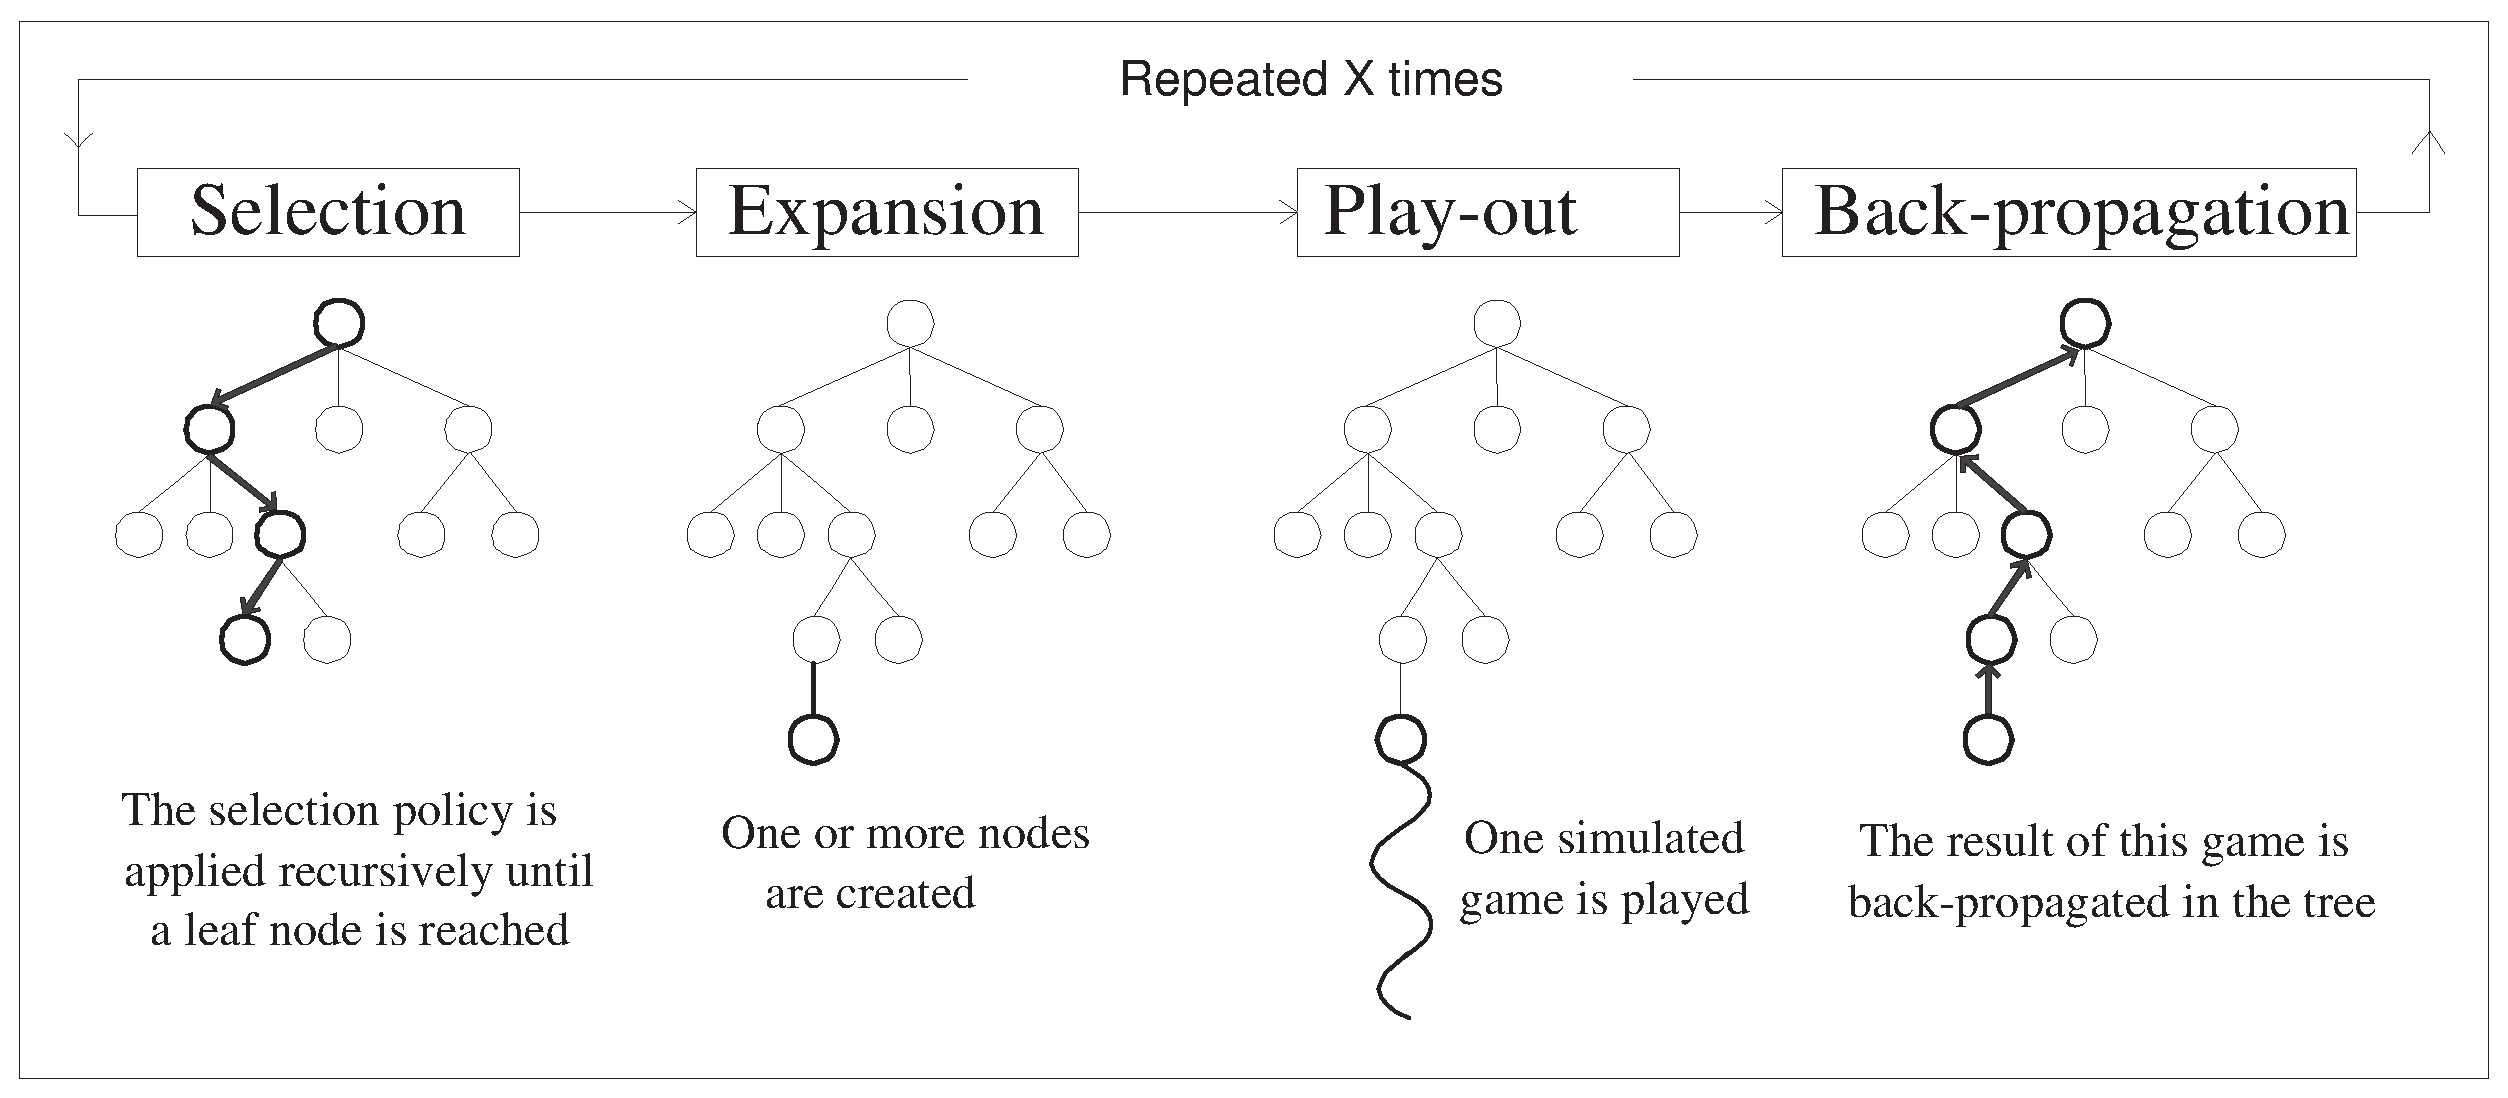
\includegraphics[width=.45\textwidth]{img/figure1.eps}
	\caption{Strategic steps of Monte-Carlo Tree Search \cite{chaslot2008progressive}.}
	\label{fig:mcts-algorithm}
\end{figure}

\section{Assessing play-out quality}
\label{sec:poqual}
In the MCTS framework, play-outs are run by finishing a single game according to a simulation strategy until a natural terminal state is reached. The result $r$ is expressed numerically in some discrete range, e.g. $r \in [-1, 0, 1]$ a loss, draw or win, respectively, and backpropagated along the tree from the expanded leaf to the root node. Other techniques have been proposed \cite{Winands2010a}, where play-outs are cut-off early and their state heuristically evaluated. Furthermore, evaluating the final score of a game has shown to improve results in score based games. However, for some domains a strong heuristic evaluation may not be available or too time-consuming, and certainly not all games determine the winning player on the highest scoring player. Nonetheless, using the straightforward discrete reward $r$, all information regarding the quality of the play-out's final position is lost. For these reasons, we propose assessing the rewards of play-outs based on information other than the loss, draw, or win state of the final position.

\begin{figure}[ht]
	\centering
	\includegraphics[width=.3\textwidth]{img/figure2.png}
	\caption{A single MCTS simulation \cite{finnsson2010learning}.}
	\label{fig:mcts-simulation}
\end{figure}

The first, straightforward assessment of a play-out's quality is the length of the game played. Consider a single MCTS simulation as depicted in Figure \ref{fig:mcts-simulation}, we can define two seperate distances: 
\begin{enumerate}
\item the number of moves from the root $S$ to the expanded leaf $N$, $d_{SN}$,
\item the number of moves required to reach $T$, the terminal state, from $N$ during play-out $p_T$.
\end{enumerate}
The length of the simulation is defined as the sum of these distances $m_{ST} = d_{SN} + p_{NT}$, i.e. the total number of moves made by both players to reach the terminal state of the game from the current gamestate.

Considering that, in Monte-Carlo methods a random element is present in simulations, each move played increases the uncertainty of the final result. The most important benefit of using this information is that it can be obtained independent of the domain. Unless the game has a fixed-length, the variance of the length of a play-out can be informative in determining its quality.

\section{Quality-based play-out rewards}
\subsection{Relative Bonus}
\subsection{Qualitative Bonus}

\section{Algorithm}

\begin{algorithm2e}[t]
  {\bf MCTS}(node $p$, cumulative node depth $d_{S, p}$):\;
  \pushline
    \If{isLeaf($p$)}{Expand($p$)}
    Select a child $c_i$ that maximizes $X_i$ from Eq.~\ref{eq:uct} \;
    \If{$n_i = 0$}{
    	$\{q_t, w_t, m_t, r_t\} \gets$ Playout$(c_i)$ 			\;			\label{alg:results}
    	
    	\If{enabled$(rb)$}{
    		$r_t \gets r_t + \sgn{r} * BONUS(\bar{M} - m_t, s_m)$ 		\;
    		Update $\bar{M}$ and $s_m$ with $m_t$							\;
		}

		\If{enabled$(qb)$} {
    		$r_t \gets r_t + \sgn{r} * BONUS(\bar{Q} - q_t, s_q)$ 		\;
    		Update $\bar{Q}$ and $s_q$ with $q_t$ 						\;
    	}
    } \Else {
    	$r_t$ = -MCTS($c_i$, $d_{S, c_i})$)						\; 
    }

    {\bf return} $r_t$												\;
  	
  	\popline
  	\;
    {\bf BONUS}(distance to mean $\delta$, sample std.dev $s$):		\;
    
    \pushline
    	$\lambda \gets \frac{\delta}{s_m}$					\;
    	$b \gets \frac{0.5}{1+\exp{-K\lambda}} - 0.25$			\;
    \bf{return} $b$											\;
    \popline

    % \ElseIf{ExpandableNode$(p,l)$}{                           \label{alg:expandstart}
    %   \For{$c \in C(p)$}{                                       \label{alg:oldnewstart}
    %     $c \gets $NewLeafNode() \;                              
    %     Add new leaf $c$ to the tree\;                          \label{alg:oldnewend}
    %   }
    %   $(R,c') \gets \mbox{Play-out}(p)$\;
    %   Update$(c,R)$; Update$(p,R)$ \;
    %   {\bf return} $(p,R)$                            \label{alg:expandend}
    % }
    % \Else{  
    %   Let $t$ be the tactic set at the root \;                          \label{alg:internalstart}
    %   $n_p \gets p.n_{old} + p.n_{new}$\;
    %   \For{$c \in C(p)$}{
    %     Let $i$ be the action associated with child $c$ \;
    %     $n_i \gets c.n_{old} + c.n_{new}$ \;
    %     $v_i \gets M^i_t$ as defined in Eq.~\ref{eq:vi}\;
    %   }
    %   Select a move $i$ that maximizes $X_i$ from Eq.~\ref{eq:uct} \;
    %   $(c, R', \Delta l) \gets p.\mbox{ApplyMove}(i)$\;                  \label{alg:transition}
    %   \If{$R'_{survival} = 0$}{                                            \label{alg:deathstart}
    %     $(R,c) \gets \mbox{Play-out}(p)$\;
    %     Update$(p,R)$\;
    %     {\bf return} $(p,R)$\;                                  		\label{alg:deathend}
    %   }
    %   $R \gets \mbox{MCTS}(c, l + \Delta l)$\;                               \label{alg:reccall}
    %   Update$(p,R)$\;
    %   {\bf return} $(p,R)$\;
    % }
  \vspace{0.3cm}
  \caption{Pseudo-code of the MCTS and BONUS functions \label{alg}}
\end{algorithm2e}

\section{Experiments}
\subsection{Experimental setup}

\subsection{Results}

\section{Conclusion}

\bibliography{references}
\end{document}